\exercise{9\textbar 1}{Entscheidung bei Handlungsalternativen}
Ein Unternehmen muss sich zwischen den beiden folgenden Handlungsalternativen entscheiden:

\begin{itemize}
    \item \textbf{A:} Beibehaltung des bisherigen Sortiments
    \item \textbf{B:} Ergänzung des bisherigen Sortiments durch ein neues Produkt
\end{itemize}

Alternative A bringt mit absoluter Sicherheit einen Gewinn von 50 €.
Der Erfolg der Alternative B dagegen ist ungewiss. Mit einer Eintrittswahrscheinlichkeit von $g = 0,20$ wird ein Gewinn in Höhe von 2.000 € erwartet. Mit größerer Wahrscheinlichkeit ($v = 0,80$) muss dagegen mit einem Verlust in Höhe von 400 € gerechnet werden.

\begin{enumerate}[label=(\alph*)]
    \item Wie groß ist der mathematische Erwartungswert des Erfolges aus Handlungsalternative B?
    \item Soll sich der Betrieb für Alternative A oder B entscheiden? Begründen Sie Ihre Antwort.
\end{enumerate}

\solution{

\begin{enumerate}[label=(\alph*)]
    \item \textbf{Mathematischer Erwartungswert für Alternative B:}

    Der mathematische Erwartungswert $E(B)$ wird berechnet, indem die möglichen Gewinne und Verluste mit ihren jeweiligen Wahrscheinlichkeiten gewichtet und anschließend summiert werden:

    \[
    E(B) = g \cdot \text{Gewinn} + v \cdot \text{Verlust}
    \]

    Einsetzen der Werte:

    \[
    E(B) = 0,20 \cdot 2.000 + 0,80 \cdot (-400)
    \]

    Berechnung:

    \[
    E(B) = 400 - 320 = 80
    \]

    Der mathematische Erwartungswert für Alternative B beträgt 80 €.

    \item \textbf{Entscheidung zwischen Alternative A und B:}

    Alternative A bietet einen sicheren Gewinn von 50 €.
    Alternative B hat einen mathematischen Erwartungswert von 80 €, jedoch ist der Erfolg unsicher, da auch ein Verlust von 400 € möglich ist.

    \textbf{Empfehlung:} Der Betrieb sollte sich für Alternative B entscheiden, da der mathematische Erwartungswert höher ist als der sichere Gewinn aus Alternative A. Allerdings hängt die Entscheidung auch von der Risikobereitschaft des Unternehmens ab. Ein risikoscheues Unternehmen könnte aufgrund der Unsicherheit Alternative A bevorzugen.
\end{enumerate}
}

\exercise{9\textbar 2}{Entscheidungsregeln (A1)}
Die verantwortlichen Stellen eines Unternehmens stehen oft vor dem Problem, dass sie Entscheidungen treffen müssen, ohne über die dazu notwendige Sicherheit in Bezug auf deren Auswirkungen zu verfügen.\\
Für solche Situationen sind Regeln entwickelt worden, die eine Entscheidung erleichtern sollen.

\begin{enumerate}[label=(\alph*)]
    \item Erklären Sie mit dem obenstehenden Beispiel die folgenden Entscheidungsregeln:
    \begin{itemize}
        \item Maximierung des Gesamterwartungswertes
        \item Minimax-Regel
        \item Maximax-Regel
        \item Pessimismus-Optimismus-Regel
        \item Minimax-Risiko-Regel
    \end{itemize}
    \item Welche Einwände können gegen die Entscheidungsregeln vorgebracht werden?
\end{enumerate}
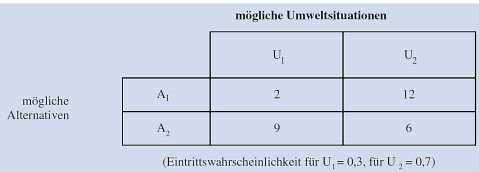
\includegraphics[width=0.6\textwidth]{figures/9_2.png}

\exercise{9\textbar 3}{Entscheidungsregeln (A2)}
Herr Unschlüssig will ein neues Produkt herstellen. Zur Wahl stehen drei Produkte, wobei Herr Unschlüssig sowohl den minimalen als auch den maximalen Gewinn kennt, der aus dem Verkauf dieser Produkte resultieren könnte.

\begin{table}[h!]
\centering
\begin{tabular}{|c|c|c|}
\hline
\textbf{Produkt} & \textbf{Minimaler Gewinn} & \textbf{Maximaler Gewinn} \\
\hline
Produkt 1 & 390 & 430 \\
\hline
Produkt 2 & 410 & 410 \\
\hline
Produkt 3 & 400 & 420 \\
\hline
\end{tabular}
\caption{Mögliche Gewinne der Produkte}
\end{table}

\begin{enumerate}[label=(\alph*)]
    \item Treffen Sie die optimale Wahl mithilfe des Hurwicz-Kriteriums (Pessimismus-Optimismus-Kriterium), wenn der Pessimismus-Optimismus-Faktor \( \alpha = 0{,}2 \) beträgt.
    \item Bestimmen Sie den kritischen Wert des Pessimismus-Optimismus-Faktors, bei dem die Alternativen „Produkt 1“ und „Produkt 2“ gerade gleichwertig sind.
    \item Beurteilen Sie dieses Verfahren.
\end{enumerate}

\solution{

\begin{enumerate}[label=(\alph*)]
    \item \textbf{Berechnung der optimalen Wahl mit dem Hurwicz-Kriterium:}

    Für das Hurwicz-Kriterium wird die Formel \( H = \alpha \cdot \text{minimaler Gewinn} + (1 - \alpha) \cdot \text{maximaler Gewinn} \) verwendet.
    
    \begin{align*}
        H_{\text{Produkt 1}} &= 0{,}8 \cdot 390 + 0{,}2 \cdot 430 = 398 \\
        H_{\text{Produkt 2}} &= 0{,}8 \cdot 410 + 0{,}2 \cdot 410 = 410 \\
        H_{\text{Produkt 3}} &= 0{,}8 \cdot 400 + 0{,}2 \cdot 420 = 404
    \end{align*}
    
    \textbf{Ergebnis:} Produkt 2 ist die optimale Wahl.

    \item \textbf{Bestimmung des kritischen Wertes von \( \alpha \):}

    Zwei Alternativen sind gleichwertig, wenn ihre Hurwicz-Werte identisch sind. Für „Produkt 1“ und „Produkt 2“ gilt:
    
    \[
    390 \cdot \alpha + 430 \cdot (1 - \alpha) = 410 \cdot \alpha + 410 \cdot (1 - \alpha)
    \]
    
    Auflösen ergibt:
    \[
    \alpha = 0{,}5
    \]

    \item \textbf{Beurteilung des Verfahrens:}
    \begin{itemize}
        \item Problem der unsicheren Informationen (Erfassung, Gewichtung) 
        \item keine Berücksichtigung der individuellen Lage des Unternehmens
        \item Risikofaktoren nur schwer einzuschätzen (nicht quantifizierbar)
        \item Keine Berücksichtigung irrationaler Faktoren
        \item Besstimmung des Pessimisum-Optimismus-Faktors ist sehr subjektiv
    \end{itemize}
\end{enumerate}
}

\exercise{9\textbar 4}{Entscheidungsregeln (A3)}
Die Möbel AG steht vor der schwierigen Entscheidung, wie sie ihr Sortiment in Zukunft gestalten soll. Drei Strategien sind möglich:

\begin{itemize}
    \item Produktion und Vertrieb von nachgebauten antiken Möbeln erster Qualität.
    \item Produktion und Vertrieb von modernen Designermöbeln der obersten Preisklasse.
    \item Produktion und Vertrieb von klassischen Möbeln mit mittlerem Preisniveau.
\end{itemize}

Die Entwicklung des Absatzes für den Möbelmarkt wird von den Marktforschungsexperten wie folgt beurteilt:
\begin{enumerate}
    \item Stetiges Wachstum des Bedarfs an Möbeln, gleiche Anbieterstruktur.
    \item Absatz wird sich wegen einer wirtschaftlichen Stagnation verringern.
    \item Stetiges Wachstum, aber verschärfte Konkurrenz unter den Anbietern.
\end{enumerate}

Die durchschnittlichen Jahresgewinne in Abhängigkeit der verschiedenen zukünftigen Marktsituationen werden wie in der unten stehenden Tabelle geschätzt (Gewinne in 1.000 €).

\begin{table}[h!]
    \centering
    \begin{tabular}{|l|c|c|c|}
        \hline
        \textbf{Strategie} & \textbf{Marktsituation 1} & \textbf{Marktsituation 2} & \textbf{Marktsituation 3} \\
        \hline
        Antike Möbel & 85 & 35 & 58 \\
        \hline
        Designermöbel & 94 & 45 & 86 \\
        \hline
        Klassische Möbel & 76 & 58 & 68 \\
        \hline
    \end{tabular}
    \caption{Gewinne je nach Marktsituation (in 1.000 €)}
    \label{tab:moebel_gewinn}
\end{table}

\begin{enumerate}[label=(\alph*)]
    \item Welche Strategie würde nach dem Minimax-Prinzip gewählt werden?
    \item Welche Strategie wählen Sie mithilfe des Maximax-Prinzips?
    \item Beurteilen Sie die beiden Verfahren.
\end{enumerate}

\solution{

\begin{enumerate}[label=(\alph*)]
    \item \textbf{Minimax-Prinzip:}
    \begin{itemize}
        \item Schritt 1: Minimalen Gewinn pro Strategie bestimmen:
        \begin{itemize}
            \item Antike Möbel: 35
            \item Designermöbel: 45
            \item Klassische Möbel: 58
        \end{itemize}
        \item Schritt 2: Variante mit dem höchsten minimalen Gewinn auswählen. Es wird die Strategie \textbf{Klassische Möbel} ausgewählt.
    \end{itemize}

    \item \textbf{Maximax-Prinzip:}
    \begin{itemize}
        \item Schritt 1: Maximalen Gewinn pro Strategie bestimmen:
        \begin{itemize}
            \item Antike Möbel: 85
            \item Designermöbel: 94
            \item Klassische Möbel: 76
        \end{itemize}
        \item Schritt 2: Variante mit dem höchsten maximalen Gewinn auswählen. Es wird die Strategie \textbf{Designermöbel} ausgewählt.
    \end{itemize}

    \item \textbf{Beurteilung der Verfahren:}
    \begin{itemize}
        \item \textbf{Allgemeine Nachteile der Entscheidungsregeln:}
        \begin{itemize}
            \item Problem der unsicheren Informationen (Erfassung, Gewichtung).
            \item Keine Berücksichtigung der individuellen Lage des Unternehmens.
            \item Risikofaktoren nur schwer einzuschätzen (nicht quantifizierbar).
            \item Keine Berücksichtigung irrationaler Faktoren.
        \end{itemize}

        \item \textbf{Spezielle Nachteile der Entscheidungsregeln:}
        \begin{itemize}
            \item \textbf{Minimax-Regel:}
            \begin{itemize}
                \item Das Risiko der Entscheidungssituation wird nicht berücksichtigt, da die verschiedenen Umweltsituationen nicht gewichtet werden.
                \item Es kann zwar das schlechteste mögliche Ergebnis eintreten, jedoch wird selten das bestmögliche Ergebnis erreicht.
            \end{itemize}
            \item \textbf{Maximax-Regel:}
            \begin{itemize}
                \item Das Risiko der Entscheidungssituation wird ebenfalls nicht berücksichtigt.
                \item Es kann zwar die Alternative mit dem bestmöglichen Ergebnis erreicht werden, jedoch meistens nur unter hohem Risiko.
            \end{itemize}
        \end{itemize}
    \end{itemize}
\end{enumerate}
}
\exercise{9\textbar 5}{Produkt-Markt-Strategien}
Beschreiben Sie am Beispiel eines Herstellers von Gummib\"archen die vier Produkt-Markt-Strategien.

\solution{

\begin{enumerate}
    \item \textbf{Marktdurchdringung:} Der Hersteller k\"onnte seine bestehenden Gummib\"archen intensiver vermarkten, z.\,B. durch Rabattaktionen oder Werbung, um die Verkaufszahlen zu steigern.
    
    \item \textbf{Marktentwicklung:} Das Unternehmen k\"onnte neue M\"arkte erschlie\"sen, indem es Gummib\"archen in L\"ander exportiert, in denen sie bisher noch nicht angeboten wurden.
    
    \item \textbf{Produktentwicklung:} Der Hersteller k\"onnte neue Varianten der Gummib\"archen entwickeln, z.\,B. mit exotischen Geschmacksrichtungen oder in Form von zuckerfreien Produkten.
    
    \item \textbf{Diversifikation:} Das Unternehmen k\"onnte komplett neue Produkte einf\"uhren, die nichts mit Gummib\"archen zu tun haben, z.\,B. Schokolade oder Snacks.
\end{enumerate}
}
\exercise{9\textbar 6}{Produkt-Markt-Strategien vs. Wettbewerbsstrategien}
Wodurch unterscheiden sich Produkt-Markt-Strategien von Wettbewerbsstrategien?

\solution{

\begin{itemize}
    \item \textbf{Produkt-Markt-Strategien:}
    \begin{itemize}
        \item Produkt-Markt-Strategien konzentrieren sich darauf, wie ein Unternehmen neue oder bestehende Produkte in bestehenden oder neuen Märkten positionieren kann.
        \item Die vier zentralen Ansätze sind:
        \begin{itemize}
            \item \textbf{Marktdurchdringung:} Steigerung des Absatzes bestehender Produkte in bestehenden Märkten.
            \item \textbf{Marktentwicklung:} Einführung bestehender Produkte in neue Märkte.
            \item \textbf{Produktentwicklung:} Entwicklung neuer Produkte für bestehende Märkte.
            \item \textbf{Diversifikation:} Einführung neuer Produkte in neue Märkte.
        \end{itemize}
    \end{itemize}

    \item \textbf{Wettbewerbsstrategien:}
    \begin{itemize}
        \item Wettbewerbsstrategien legen den Schwerpunkt darauf, wie ein Unternehmen sich gegenüber seinen Mitbewerbern in einem Markt differenzieren und positionieren kann.
        \item Die drei grundlegenden Strategien nach Porter sind:
        \begin{itemize}
            \item \textbf{Kostenführerschaft:} Minimierung der Kosten, um Produkte zu einem niedrigeren Preis als die Konkurrenz anbieten zu können.
            \item \textbf{Differenzierung:} Schaffung eines einzigartigen Wertes für Kunden, beispielsweise durch Qualität, Marke oder Service.
            \item \textbf{Fokussierung:} Konzentration auf eine spezielle Nische, entweder durch Kostenführerschaft oder Differenzierung in einem begrenzten Marktsegment.
        \end{itemize}
    \end{itemize}

    \item \textbf{Unterschiede:}
    \begin{itemize}
        \item Produkt-Markt-Strategien zielen darauf ab, Wachstumschancen zu identifizieren und Produkte und Märkte strategisch auszurichten.
        \item Wettbewerbsstrategien richten den Fokus auf die Positionierung gegenüber Wettbewerbern und die Schaffung von Wettbewerbsvorteilen.
        \item Während Produkt-Markt-Strategien primär auf die Kombination von Märkten und Produkten abzielen, betrachten Wettbewerbsstrategien die Methoden, um in diesen Märkten erfolgreich zu agieren.
    \end{itemize}
\end{itemize}
}
\exercise{9\textbar 7}{Strategische Erfolgspositionen}
Um langfristig überleben zu können, muss ein Unternehmen strategische Erfolgspositionen aufbauen.

\begin{enumerate}[label=(\alph*)]
    \item Was versteht man unter einer strategischen Erfolgsposition?
    \item Welche Bedingungen müssen erfüllt sein, damit man von einer strategischen Erfolgsposition sprechen kann?
    \item Geben Sie Beispiele für strategische Erfolgspositionen Ihnen bekannter Unternehmen.
\end{enumerate}

\solution{
\textbf{Lösung:}

\begin{enumerate}[label=(\alph*)]
    \item \textbf{Definition einer strategischen Erfolgsposition:}
    \begin{itemize}
        \item Eine strategische Erfolgsposition (SEP) beschreibt einen einzigartigen und langfristigen Wettbewerbsvorteil, den ein Unternehmen gegenüber seinen Mitbewerbern besitzt.
        \item Dieser Vorteil ermöglicht es dem Unternehmen, nachhaltig höhere Gewinne zu erzielen, indem es seine Marktposition sichert und ausbaut.
        \item SEPs basieren häufig auf schwer imitierbaren Ressourcen, Fähigkeiten oder Technologien.
    \end{itemize}

    \item \textbf{Bedingungen für eine strategische Erfolgsposition:}
    \begin{itemize}
        \item \textbf{Einzigartigkeit:} Die Position muss sich signifikant von der Konkurrenz unterscheiden.
        \item \textbf{Nachhaltigkeit:} Der Vorteil muss langfristig bestehen und schwer kopierbar sein.
        \item \textbf{Relevanz für den Kunden:} Der Vorteil muss für Kunden einen erkennbaren Mehrwert bieten.
        \item \textbf{Wirtschaftliche Rentabilität:} Die Position muss zu einem Wettbewerbsvorteil führen, der sich in höheren Gewinnen widerspiegelt.
    \end{itemize}

    \item \textbf{Beispiele für strategische Erfolgspositionen:}
    \begin{itemize}
        \item \textbf{Apple:} 
        \begin{itemize}
            \item Starkes Markenimage und hohe Kundenbindung.
            \item Innovationsführerschaft in Design und Technologie (z. B. iPhone, MacBook).
        \end{itemize}
        \item \textbf{Tesla:}
        \begin{itemize}
            \item Führende Position in der Elektromobilität.
            \item Überlegenes Batterie- und Ladesystem sowie eine starke Marke.
        \end{itemize}
        \item \textbf{Coca-Cola:}
        \begin{itemize}
            \item Weltweite Bekanntheit und Markentreue.
            \item Starkes Vertriebsnetzwerk und kontinuierliche Innovationen im Marketing.
        \end{itemize}
        \item \textbf{IKEA:}
        \begin{itemize}
            \item Effiziente Wertschöpfungskette mit Fokus auf Selbstmontage.
            \item Kombination aus niedrigen Preisen und ansprechendem skandinavischen Design.
        \end{itemize}
    \end{itemize}
\end{enumerate}
}

\exercise{9\textbar 8}{Lernkurve vs. Erfahrungskurve}
Sowohl die Lern- als auch die Erfahrungskurve ermöglichen Kostensenkungen im Betrieb.

\begin{enumerate}[label=(\alph*)]
    \item Welches ist der Unterschied zwischen der Lern- und der Erfahrungskurve?
    \item Welchen Zusammenhang sehen Sie zwischen der Erfahrungskurve und den Economies of Scale?
\end{enumerate}

\solution{

\begin{enumerate}[label=(\alph*)]
    \item \textbf{Unterschied zwischen Lern- und Erfahrungskurve:}
    \begin{itemize}
        \item \textbf{Lernkurve:}
        \begin{itemize}
            \item Beschreibt die Kostensenkung, die durch die Steigerung individueller Fähigkeiten und Effizienz bei der Wiederholung einer Tätigkeit erreicht wird.
            \item Fokus liegt auf der Produktivität der Mitarbeiter und der kontinuierlichen Verbesserung der Arbeitsabläufe.
            \item Beispiel: Ein Mitarbeiter benötigt für die Montage eines Produkts weniger Zeit, je häufiger er die Aufgabe wiederholt.
        \end{itemize}
        \item \textbf{Erfahrungskurve:}
        \begin{itemize}
            \item Betrachtet die gesamte Wertschöpfungskette und berücksichtigt Skaleneffekte, Technologieverbesserungen und organisatorisches Lernen.
            \item Besagt, dass mit jeder Verdopplung der kumulierten Produktionsmenge die Stückkosten um einen konstanten Prozentsatz sinken.
            \item Umfasst mehr Faktoren als die Lernkurve, wie zum Beispiel Automatisierung, bessere Ressourcennutzung und Innovationsprozesse.
        \end{itemize}
        \item \textbf{Zusammenfassung des Unterschieds:}
        \begin{itemize}
            \item Die Lernkurve fokussiert sich auf individuelle und arbeitsbezogene Verbesserungen.
            \item Die Erfahrungskurve bezieht sich auf unternehmensweite Effizienzsteigerungen entlang der gesamten Wertschöpfungskette.
        \end{itemize}
    \end{itemize}

    \item \textbf{Zusammenhang zwischen Erfahrungskurve und Economies of Scale:}
    \begin{itemize}
        \item Die Erfahrungskurve und die Economies of Scale sind eng miteinander verbunden, da beide Mechanismen auf Kostensenkungen durch Produktionssteigerungen abzielen.
        \item \textbf{Economies of Scale:}
        \begin{itemize}
            \item Kostenvorteile, die durch die Steigerung des Produktionsvolumens erreicht werden.
            \item Fixkosten werden auf eine größere Menge an Produkten verteilt, was die Stückkosten senkt.
        \end{itemize}
        \item \textbf{Erfahrungskurve:}
        \begin{itemize}
            \item Geht über die Economies of Scale hinaus, da sie auch Lern- und Effizienzsteigerungen durch technologische Innovationen und organisatorisches Wissen berücksichtigt.
        \end{itemize}
        \item \textbf{Zusammenhang:}
        \begin{itemize}
            \item Beide Konzepte wirken oft gemeinsam: Höhere Produktionsmengen führen zu Skaleneffekten (Economies of Scale) und fördern gleichzeitig das Sammeln von Erfahrungen, die zusätzliche Kostensenkungen ermöglichen.
            \item Beispiel: In der Automobilproduktion können große Stückzahlen (Economies of Scale) die Fixkosten senken, während gleichzeitig Prozessinnovationen (Erfahrungskurve) die variablen Kosten reduzieren.
        \end{itemize}
    \end{itemize}
\end{enumerate}
}

\exercise{9\textbar 9}{Wettbewerbsstrategien}
Wettbewerbsstrategien sollen es dem Unternehmen ermöglichen, sich gegenüber der Konkurrenz im Markt zu behaupten, indem sie einen erfolgreichen Umgang mit den Wettbewerbskräften erlauben.

\begin{enumerate}[label=(\alph*)]
    \item Welche Wettbewerbsstrategien unterscheidet Porter?
    \item Zeigen Sie, welche Gefahren und Risiken mit den verschiedenen Wettbewerbsstrategien verbunden sind.
\end{enumerate}

\solution{
\textbf{Lösung:}

\begin{enumerate}[label=(\alph*)]
    \item \textbf{Wettbewerbsstrategien nach Porter:}
    Michael E. Porter unterscheidet in seinem Modell drei generische Wettbewerbsstrategien, die Unternehmen nutzen können, um Wettbewerbsvorteile zu erzielen:
    \begin{itemize}
        \item \textbf{Kostenführerschaft:}
        \begin{itemize}
            \item Ziel ist es, durch geringe Kosten und eine effiziente Produktion die niedrigsten Preise im Markt anzubieten.
            \item Beispiele: Einsatz von Skaleneffekten, Standardisierung, Automatisierung.
        \end{itemize}
        \item \textbf{Differenzierung:}
        \begin{itemize}
            \item Ziel ist es, sich durch einzigartige Produkte oder Dienstleistungen von der Konkurrenz abzuheben.
            \item Beispiele: Markenbildung, Produktinnovationen, hoher Kundenservice.
        \end{itemize}
        \item \textbf{Fokussierung:}
        \begin{itemize}
            \item Konzentration auf eine bestimmte Nische oder ein Marktsegment.
            \item Ziel ist es, in diesem Bereich entweder Kostenführerschaft oder Differenzierung zu erreichen.
        \end{itemize}
    \end{itemize}

    \item \textbf{Gefahren und Risiken der Wettbewerbsstrategien:}
    \begin{itemize}
        \item \textbf{Kostenführerschaft:}
        \begin{itemize}
            \item \textbf{Gefahr der Preiskriege:} Wettbewerber können ebenfalls die Preise senken, wodurch die Margen stark schrumpfen.
            \item \textbf{Qualitätsprobleme:} Starke Kostenreduktionen können zu einer Verschlechterung der Produkt- oder Servicequalität führen.
            \item \textbf{Abhängigkeit von Skaleneffekten:} Ein Rückgang der Nachfrage kann die Kostenvorteile gefährden.
        \end{itemize}
        \item \textbf{Differenzierung:}
        \begin{itemize}
            \item \textbf{Hohe Kosten:} Differenzierung erfordert oft erhebliche Investitionen in Forschung, Entwicklung und Marketing.
            \item \textbf{Nachahmung durch Wettbewerber:} Einzigartige Merkmale können kopiert werden, wodurch der Differenzierungsvorteil verloren geht.
            \item \textbf{Marktveränderungen:} Kundenpräferenzen können sich ändern, wodurch die Differenzierungsstrategie unwirksam wird.
        \end{itemize}
        \item \textbf{Fokussierung:}
        \begin{itemize}
            \item \textbf{Begrenztes Marktpotenzial:} Die Zielgruppe ist oft klein, was das Wachstum einschränkt.
            \item \textbf{Abhängigkeit von der Nische:} Veränderungen in der Nische können existenzbedrohend sein.
            \item \textbf{Angriffe durch größere Unternehmen:} Große Anbieter können die Nische ebenfalls bedienen und kleinere Wettbewerber verdrängen.
        \end{itemize}
    \end{itemize}
\end{enumerate}
}

\exercise{9\textbar 10}{Wettbewerbskräfte, Wettbewerbsstrategie und Preisstrategie}
Die Panorama AG ist im Pharmabereich tätig. 40~\% des Umsatzes werden mit Erkältungsmitteln, weitere 35~\% mit Schlafmitteln und die restlichen 25~\% mit Aufbaupräparaten erzielt.

Mit 250 Mitarbeitenden wird ein Jahresumsatz von 32 Mio. € erzielt, der zu fast 100~\% in Deutschland erarbeitet wird. Der Cashflow beträgt 4,2 Mio. €.

Das Unternehmen beabsichtigt, ein von ihm selbst entwickeltes Medikament zu lancieren. Das neue Produkt dient der Vorbeugung gegen Erkältungskrankheiten und kann das ganze Jahr hindurch eingenommen werden.

Marktuntersuchungen haben ergeben, dass zwei bis drei Jahre nach der Lancierung mit einem Marktanteil von 5~\% gerechnet werden kann. Es ist nicht damit zu rechnen, dass der Marktanteil in ferner Zukunft wesentlich vergrößert werden kann.

\begin{enumerate}[label=(\alph*)]
    \item Welchen Wettbewerbskräften sieht sich das Unternehmen bei der Markteinführung seines neuen Produktes gegenüber?
    \item Welche Wettbewerbsstrategie für das neue Produkt würden Sie dem Unternehmen empfehlen?
    \item Auf welche Erhebungstechnik könnte die Panorama AG ihre Marktforschung gestützt haben?
    \item Nach welchen Kriterien wird die Preisstrategie für das neue Medikament zu wählen sein?
\end{enumerate}

\solution{
\textbf{Lösung:}

\begin{enumerate}[label=(\alph*)]
    \item \textbf{Wettbewerbskräfte nach Porter:}
    Die Panorama AG sieht sich bei der Markteinführung des neuen Produkts den folgenden Wettbewerbskräften gegenüber:
    \begin{itemize}
        \item Verhandlungsmacht der Abnehmer.
        \item Verhandlungsmacht der Lieferanten.
        \item Bedrohung durch Ersatzprodukte und -dienste.
        \item Bedrohung durch neue Konkurrenten.
        \item Rivalität unter den bestehenden Unternehmen.
    \end{itemize}

    \item \textbf{Empfohlene Wettbewerbsstrategie:}
    \begin{itemize}
        \item Die Panorama AG betreibt bereits eine Nischenstrategie in Bezug auf ihre bisherigen Produkte.
        \item Da mit dem neuen Produkt nur ein Marktanteil von 5~\% zu rechnen ist und das Unternehmen bereits im Marktsegment „Erkältungsmittel“ tätig ist, bietet sich eine \textbf{Nischenstrategie} für das neue Produkt in diesem Segment an.
        \item Gleichzeitig könnte eine \textbf{Differenzierungsstrategie} verfolgt werden, da die geringe Größe des Marktanteils wenig Raum für Economies of Scale lässt und damit die Kostenführerschaft erschwert wird.
        \item Zusätzliche Faktoren wie kartellähnliche Strukturen in der Medikamentenbranche könnten die Wahl einer Kostenführerschaft-Strategie zusätzlich einschränken.
    \end{itemize}

    \item \textbf{Erhebungsmethoden:}
    Die Panorama AG könnte ihre Marktforschung auf folgende Erhebungsansätze gestützt haben:
    \begin{itemize}
        \item \textbf{Primärforschung:}
        \begin{itemize}
            \item Befragungen von Endverbrauchern, um die Akzeptanz des neuen Medikaments zu ermitteln.
            \item Interviews mit Fachleuten, z. B. Ärzten oder Apothekern, die die Verschreibung und Empfehlung beeinflussen.
        \end{itemize}
        \item \textbf{Sekundärforschung:}
        \begin{itemize}
            \item Analyse von bestehenden Marktstudien und Daten zur Nachfrage nach Erkältungsmedikamenten.
            \item Untersuchung von Wettbewerbsprodukten und deren Marktposition.
        \end{itemize}
    \end{itemize}

    \item \textbf{Kriterien zur Preisstrategie:}
    Die Preisstrategie für das neue Medikament sollte auf den folgenden Kriterien basieren:
    \begin{itemize}
        \item \textbf{Kostenbasierte Preisgestaltung:}
        \begin{itemize}
            \item Berücksichtigung der Produktionskosten sowie Forschung und Entwicklung.
        \end{itemize}
        \item \textbf{Wettbewerbsorientierte Preisgestaltung:}
        \begin{itemize}
            \item Analyse der Preise vergleichbarer Produkte auf dem Markt.
            \item Positionierung des Preises, um sich von Konkurrenzprodukten abzuheben.
        \end{itemize}
        \item \textbf{Wertorientierte Preisgestaltung:}
        \begin{itemize}
            \item Wahrnehmung des Kundennutzens, z. B. Prävention von Erkältungskrankheiten und einfache Anwendung.
        \end{itemize}
    \end{itemize}
\end{enumerate}
}

\exercise{9\textbar 11}{Kurzfristige Planung bei unsicherer Wirtschaftslage}
Nehmen Sie zur folgenden Aussage Stellung:
\begin{quote}
    „Je unsicherer die Wirtschaftslage ist, umso kurzfristiger muss die Planung sein.“
\end{quote}

\solution{

Die Aussage, „Je unsicherer die Wirtschaftslage ist, umso kurzfristiger muss die Planung sein“, lässt sich wie folgt bewerten:

\begin{itemize}
    \item \textbf{Begründung für kurzfristige Planung:}
    \begin{itemize}
        \item \textbf{Flexibilität:} Unsichere Wirtschaftslagen erfordern schnelle Reaktionen auf Änderungen in den Marktbedingungen, wie z. B. Schwankungen der Nachfrage oder Rohstoffpreise.
        \item \textbf{Risikominimierung:} Längerfristige Planungen bergen ein höheres Risiko von Fehlentscheidungen, da unvorhergesehene Ereignisse (z. B. Krisen oder wirtschaftliche Einbrüche) die Planungsgrundlage verändern können.
        \item \textbf{Kostenkontrolle:} Kurzfristige Planung ermöglicht es, Budgets und Investitionen besser an aktuelle Gegebenheiten anzupassen und so unnötige Kosten zu vermeiden.
    \end{itemize}

    \item \textbf{Gegenargumente:}
    \begin{itemize}
        \item \textbf{Langfristige Perspektive:} Auch in unsicheren Zeiten ist eine langfristige Planung wichtig, um strategische Ziele nicht aus den Augen zu verlieren. Dies betrifft insbesondere Investitionen in Forschung und Entwicklung oder den Aufbau neuer Märkte.
        \item \textbf{Planungsunsicherheit:} Kurzfristige Planungen können dazu führen, dass Entscheidungen zu oft geändert werden müssen, was wiederum zu Instabilität und Ineffizienz führt.
    \end{itemize}

    \item \textbf{Kombination aus kurz- und langfristiger Planung:}
    \begin{itemize}
        \item \textbf{Szenarioplanung:} Unsichere Wirtschaftslagen können mit einer Kombination aus kurz- und langfristigen Plänen bewältigt werden, indem alternative Szenarien berücksichtigt werden.
        \item \textbf{Rollierende Planung:} Ein Ansatz, der regelmäßige Anpassungen der langfristigen Planung vorsieht, kann Unsicherheiten besser abfedern.
    \end{itemize}

    \item \textbf{Fazit:}
    Die Aussage ist nicht uneingeschränkt gültig. Während eine kurzfristige Planung in unsicheren Wirtschaftslagen Vorteile bietet, bleibt eine langfristige Perspektive für die Sicherung der Wettbewerbsfähigkeit und strategischen Ausrichtung des Unternehmens essenziell. Eine ausgewogene Kombination aus beiden Ansätzen ist der effektivste Weg, um Unsicherheiten zu begegnen.
\end{itemize}
}

